\definecolor{keywordstyle}{rgb}{0,0,0.82}
\definecolor{commentstyle}{rgb}{0,0.6,0}
\definecolor{numberstyle}{rgb}{0.5,0.5,0.5}
\definecolor{stringstyle}{rgb}{0.58,0,0.82}

\chapter{Tools}
\label{chap:Tools}

In this chapter, the most important tools used in this work will be presented.
All the tools that were developed for this thesis are available at
\url{https://github.com/Accacio/docsTCC/tree/master/tools}. The development of
these tools was made using Ubuntu 18.04, wrapping some linux and Unix
programs/utilities, 100\% compatibility with other operating systems/platforms
was not the primary objective of this part of the work, but can be performed in
some future work.

\section{Daoct}
\label{sec:daoct}

To implement the algorithm \ref{alg:identification}, as seen in
\cite{moreira2018enhanced}, a script was created by Ryan Pitanga as part of his
undergraduate thesis, \cite{pitanga2019modelo}. His code was partially
reimplemented, so it could be used as a command line tool based in common Linux
utils (using stdin and
stdout\footnote{\url{http://man7.org/linux/man-pages/man3/stdin.3.html}}, very
useful to pipe\footnote{\url{http://man7.org/linux/man-pages/man2/pipe.2.html}}
processes). Another modification, was to change the csv input file format,
figure \ref{fig:daoctInput}, so the
program could be generic, the names of the variables (inputs and outputs) are in
the header, making the program more generic. One extra feature was added,
now the automaton generated by the algorithm can be printed to stdout in the
dot\footnote{format used by the program graphviz (\url{https://graphviz.org/})
  to draw graphs} file format, this output can be treated by one of the further
described scripts to draw the automatons shown on this thesis \todo{referenciar
  pelo menos uma figura de automato}. \doing{Also there is an option to print
  the automaton in a list of \ffunction, as seen in \todo{quando usar a lista
    citar pelo menos um aqui}}
An example of the output of the help option can be seen in \ref{fig:daoctHelp}

\todo{ change figure\begin{figure}[H]
  \centering 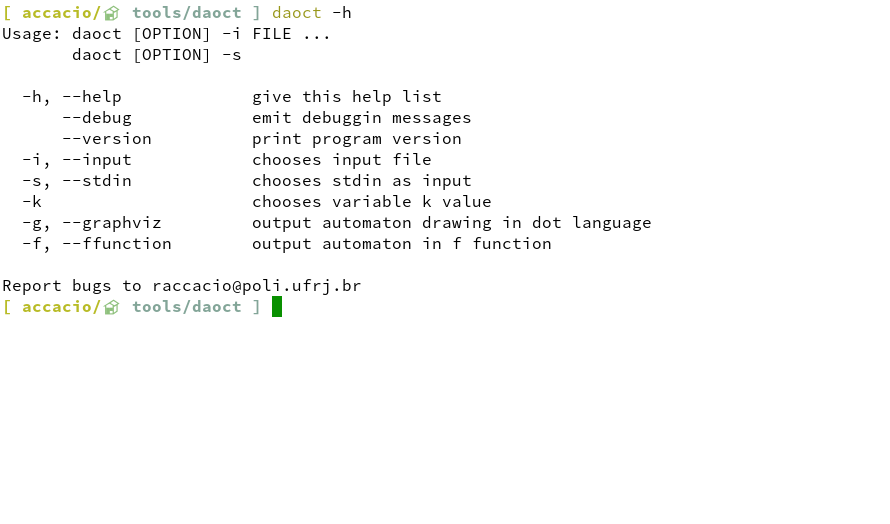
\includegraphics[trim={0 12cm 0cm
    0},clip,width=\textwidth]{tools/daoct/daoctHelp.png}
  \caption{Daoct help dialog.}
  \label{fig:daoctHelp}
\end{figure}}

An example of a csv input and the script's different outputs can
be seen in the following figures:

\begin{figure}[H]
\begin{minipage}[H]{0.5\textwidth}
  \centering 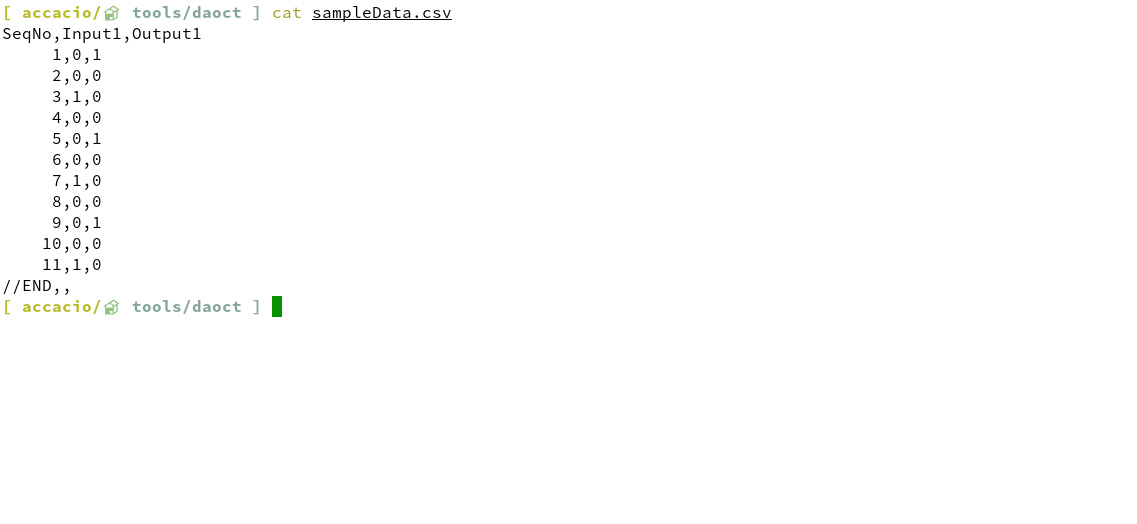
\includegraphics[trim={0 10cm 17cm
    0},clip,width=0.9\textwidth]{tools/daoct/daoctInput.png}
  \caption{Daoct input csv file.}
  \label{fig:daoctInput}
\end{minipage}
\begin{minipage}[H]{0.5\textwidth}
  \centering 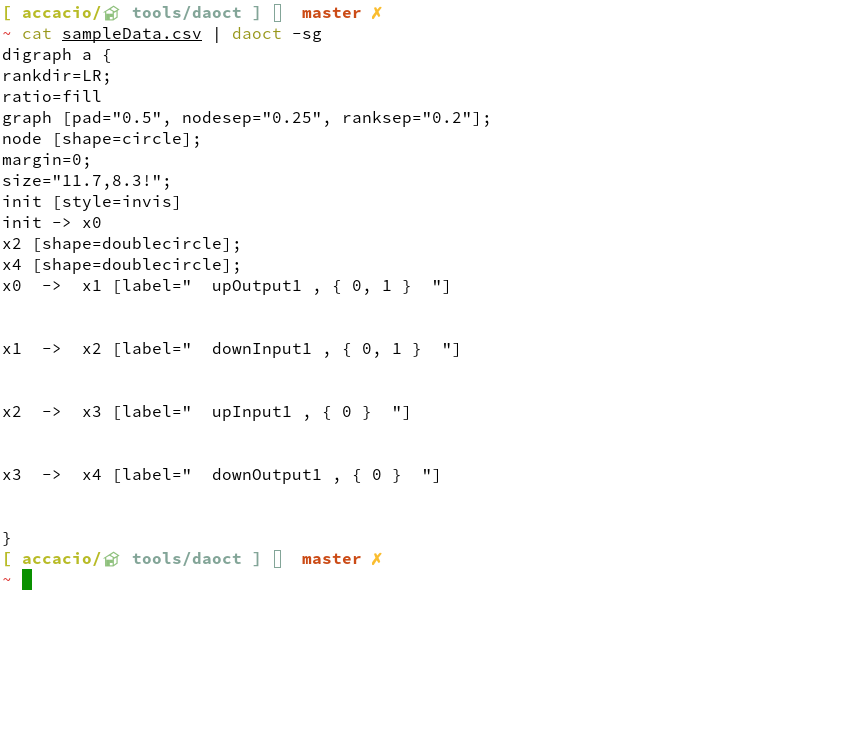
\includegraphics[trim={0 5cm 13.5cm
    0},clip,width=0.9\textwidth]{tools/daoct/daoctOutput.png}
  \caption{Daoct graphviz output.}
  \label{fig:daoctOutput}
\end{minipage}
\end{figure}  

\todo{fazer imagem com lista de \ffunction{} e colocar aqui
\figplaceholder{List of \ffunction{} output}{daoctOutputFfunction}
}

% \lstinputlisting[caption=daoct
% main,language=Python]{../../tools/python/DAOCT/daoct}

% \definecolor{keywordstyle}{rgb}{0,1,0.82} \lstinputlisting[caption=daoct
% ,language=Python]{../../tools/python/DAOCT/daoct.py}

% \lstinputlisting[caption=Utils
% ,language=Python]{../../tools/python/DAOCT/utils.py}

% \lstinputlisting[caption=Automaton
% ,language=Python]{../../tools/python/DAOCT/automaton.py}

\section{dot2automata}
\label{sec:dot2automata}

% \lstinputlisting[caption=configPetriNet,language=bash]{../../tools/bash/configPetriNet}

% \lstinputlisting[caption=dot2automata,language=bash]{../../tools/bash/dot2automata}

% \lstinputlisting[caption=dot2petri,language=bash]{../../tools/bash/dot2petri}

% \lstinputlisting[caption=linkPetriNets,language=bash]{../../tools/bash/linkPetriNets}

% \lstinputlisting[caption=linkTables,language=bash]{../../tools/bash/linkTables}

% \lstinputlisting[caption=petriml2dot,language=bash]{../../tools/bash/petriml2dot}

% \lstinputlisting[caption=removeVarsFromData,language=bash]{../../tools/bash/removeVarsFromData}

% \lstinputlisting[caption=treatCSV,language=bash]{../../tools/bash/treatCSV}






%%% Local Variables:
%%% mode: latex
%%% TeX-master: "../monografia"
%%% End:
